\section{Interpolation}

\textbf{ISOContours}: all points lying on the same line with the same values \\
\textbf{Goal of interpolation}: construct continuous function $f$ which approximates given values

\subsection{Radial Basis Functions}
Each point $(p_i, f_i)$ influences $f(x)$ based on distance: \\
$$r = \Vert p_i - x \Vert$$
$$f(x) = \sum_{i = 1}^{N} f_i \cdot \varphi(\Vert p_i - x \Vert)$$
$$\varphi(r) = e^{-r^2}$$

\textbf{Weighted radial basis functions}

$f(p_j)$ interpolates the value $f_j$

$$f(p_j) = \sum_{i = 1}^N w_i \cdot \varphi (\Vert p_i - p_j \Vert) = f_j$$

Yields a system of linear equations to be solved for $w_i$:

$$
    A = \begin{pmatrix}
        \varphi(\Vert p_1 - p_1 \Vert) & \cdots & \varphi(\Vert p_N - p_1 \Vert) \\
        \vdots                         & \ddots & \vdots                         \\
        \varphi(\Vert p_1 - p_N \Vert) & \cdots & \varphi(\Vert p_N - p_N \Vert)
    \end{pmatrix}
$$
$$
    W = \begin{bmatrix}
        w_1 \\ \vdots \\ w_N
    \end{bmatrix}
    F = \begin{bmatrix}
        f_1 \\ \vdots \\ f_N
    \end{bmatrix}
$$
$$W = A^{-1} \cdot F$$

\textbf{Drawbacks}: global influence of every sample, adding a new point requires solving the equation system, computationally expensive

\textbf{Inverse Distance Weighting}

\textbf{Assumption}: Nearby points are more similar than those further away.

$$f(x) = \sum_{i = 1}^N f_i \varphi(\Vert p_i - x \Vert)$$
$$d_i = \Vert p_i - x \Vert \hspace{1cm}
    \varphi(r) = \frac{\frac{1}{r^2}}{\sum_{i = 1}^N \frac{1}{d_i^2}}$$

\textbf{Adjusted formula}:
$$\sum_{i = 1}^N \frac{f_i}{\Vert p_i - x \Vert ^2} / \sum_{i = 1}^N \frac{1}{\Vert p_i - x \Vert ^2}$$

\textbf{Drawbacks}: still costly, still global influence of every sample

\subsection{Triangulation}
Giving up smooth, precise reconstruction in favor of speed

\textbf{Generating a Triangulation}

\textbf{Goals}: avoid long and thin triangles, maximize minimum angle in the triangulation, maximize $\frac{\text{radius of circle}}{\text{radius of circumcircle}}$

\textbf{Delaunay Triangulation}

\textbf{1}. Circumcircle does not contain another point of the set \\
\textbf{2}. Maximizes minimum angle of triangulation \\
\textbf{3}. Triangulation is unique for all but trivial cases

\textbf{Voronoi Diagram}

\begin{filecontents*}{voronoiPoints.dat}
    1.645370 0.643096
    -0.658113 1.655264
    -0.135778 -0.651569
\end{filecontents*}

\begin{filecontents*}{voronoiTriPoints.dat}
    -0.135778 -0.651569
    -0.658113 1.655264
    1.645370 0.643096
    -0.135778 -0.651569
\end{filecontents*}

\begin{filecontents*}{voronoi.dat}
    0.276155 0.654257
    -3.162349 -0.124321

    0.276155 0.654257
    1.694429 3.881949

    0.276155 0.654257
    2.349036 -2.197525

    0.276155 0.654257
    -3.162349 -0.124321
\end{filecontents*}

\begin{center}
    \begin{tikzpicture}[thick,scale=0.6, every node/.style={scale=0.6}]
        \begin{axis}[
                axis equal image,
                xtick=\empty,
                ytick=\empty,
                set layers
            ]
            \addplot [only marks, red] table {voronoiPoints.dat};
            \addplot [no markers, blue,name path=triangle] table {voronoiTriPoints.dat};
            \addplot [no markers, update limits=false,name path=lines] table {voronoi.dat};
            \node[below=2pt]
            at (axis cs:-0.135778,-0.651569)
            {$a$};
            \node[left=2pt]
            at (axis cs:-0.658113,1.655264)
            {$b$};
            \node[right=2pt]
            at (axis cs:1.645370,0.643096)
            {$c$};
            \clip[on layer=axis grid]
            (axis cs:-0.135778,-0.651569) --
            (axis cs:-0.658113,1.655264) --
            (axis cs:1.645370,0.643096) --
            (axis cs:-0.135778,-0.651569) -- cycle;
            \addplot fill between[
                    on layer=main,
                    of=triangle and lines,
                    split,
                    every segment no 0/.style={blue,fill opacity=0},
                    every segment no 1/.style={yellow,fill opacity=0.25},
                    every segment no 2/.style={red,fill opacity=0.25},
                    every segment no 3/.style={green,fill opacity=0.25},
                ];
        \end{axis}
    \end{tikzpicture}
\end{center}

Every \textbf{Voronoi Sample} ($a, b, c$) is a vertex of a \textbf{Delaunay} triangulation

\subsection{Interpolation Inside a Triangle}
\begin{center}
    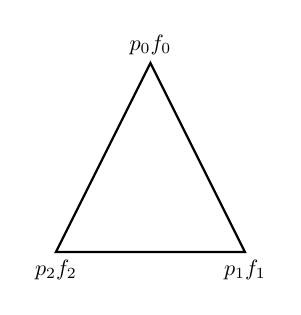
\begin{tikzpicture}[thick,scale=0.6, every node/.style={scale=0.8}]
        \draw (0,0) node[anchor=north]{$p_2 f_2$}
        -- (2,4) node[anchor=south]{$p_0 f_0$}
        -- (4,0) node[anchor=north]{$p_1 f_1$}
        -- cycle;
    \end{tikzpicture}
\end{center}

Find a function $f$ that interpolates $f_i$ at the point $p_i$ such that:

$$f(p_i) = f_i \hspace{1cm} i = 0, \cdots, N$$

Linear function:
$$f(x) = a + bx + cy$$

Where $a, b, c$ can be obtained with:

$$
    X = \begin{pmatrix}
        1 & x_0 & y_0 \\
        1 & x_1 & y_1 \\
        1 & x_2 & y_2 \\
    \end{pmatrix}
    A = \begin{bmatrix}
        a \\ b \\ c
    \end{bmatrix}
    F = \begin{bmatrix}
        f_0 \\ f_1 \\ f_2
    \end{bmatrix}
$$

$$A = X^{-1} \cdot F$$

\subsection{Baricentric Interpolation}

We want to have a smooth, continuous interpolation $\forall \alpha \in [0, 1]$

$$f(\alpha) = \alpha \cdot p_0 + (1 - \alpha) \cdot p_0$$

\begin{center}
    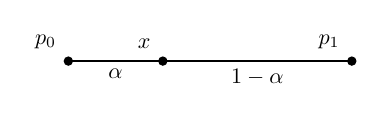
\begin{tikzpicture}[thick,scale=0.8, every node/.style={scale=0.8}]
        \tikzset{
            mydot/.style={
                    fill,
                    circle,
                    inner sep=1.5pt
                }
        }
        \path (0:4.5) coordinate (A) (0:1.5) coordinate (B) (0:0) coordinate (C);
        \draw (A)
        -- (B) node [midway, below]{$1 - \alpha$} -- (C) node [midway, below]{$\alpha$}  -- (A) -- cycle;
        \node[mydot,label={above left:$p_1$}] at (A) {};
        \node[mydot,label={above left:$x$}] at (B) {};
        \node[mydot,label={above left:$p_0$}] at (C) {};
        % \draw[|<->|] ($(A)!10mm!90:(C)$)--node[fill=white] {$z$} ($(C)!10mm!-90:(A)$);
    \end{tikzpicture}
\end{center}

$$\alpha_0 = A_0 / A , \ \alpha_1 = A_1 / A , \ \alpha_2 = A_2 / A$$
Where $A =$ area of the triangle
$$x = \alpha_0 p_0 + \alpha_1 p_1 + \alpha_2 p_2$$
$$\alpha_0 + \alpha_1 + \alpha_2 = 1$$

If $\alpha_i$ are known, then $f(x)$ can be interpolated from values $f_i$ at the vertices via:

$$f(x) = \alpha_0 f_0 + \alpha_1 f_1 + (1 - \alpha_0 - \alpha1) \cdot f_2$$

Given a point $Q$ we can find $\alpha$ by solving the linear system:

$$P = \begin{pmatrix}
        p_{0x} & p_{1x} & p_{2x} \\
        p_{0y} & p_{1y} & p_{2y} \\
        1      & 1      & 1      \\
    \end{pmatrix}$$
$$A = \begin{bmatrix}
        \alpha_0 \\ \alpha_1 \\ \alpha_2
    \end{bmatrix} X = \begin{bmatrix}
        Q_x \\ Q_y \\ 1
    \end{bmatrix}$$

$$A = P^{-1} \cdot X$$

\subsection{Scalar Interpolation}
Formula of tetrahedron:
$$f(x) = a + bx + cy + dz$$

\begin{center}
    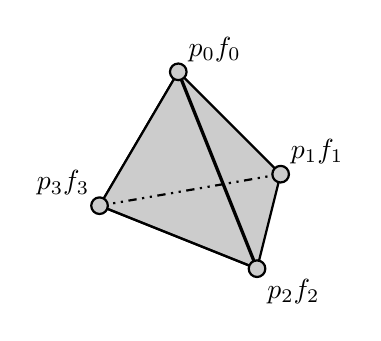
\begin{tikzpicture}

        \coordinate (a) at (4,2.5);
        \coordinate (b) at (3,.8);
        \coordinate (c) at (5,0);
        \coordinate (d) at (5.3,1.2);

        \draw[thick, fill=black!10] (a) -- (b) -- cycle;
        \draw[thick, fill=black!20] (a) -- (b) -- (c) -- (d) -- cycle;
        \draw[thick, fill=black!30] (b) -- (c) -- cycle;
        \draw[very thick] (a) -- (c);
        \draw[thick, dash dot dot] (b) -- (d);

        \fill[black!20, draw=black, thick] (a) circle (3pt) node[black, above right] {$p_0 f_0$};
        \fill[black!20, draw=black, thick] (b) circle (3pt) node[black, above left] {$p_3 f_3$};
        \fill[black!20, draw=black, thick] (c) circle (3pt) node[black, below right] {$p_2 f_2$};
        \fill[black!20, draw=black, thick] (d) circle (3pt) node[black, above right] {$p_1 f_1$};

    \end{tikzpicture}
\end{center}

Can get values $a, b, c, d$ by solving linear system:

$$X = \begin{pmatrix}
        1 & x_0 & y_0 & z_0 \\
        1 & x_1 & y_1 & z_1 \\
        1 & x_2 & y_2 & z_2 \\
        1 & x_3 & y_3 & z_3 \\
    \end{pmatrix}$$
$$A = \begin{bmatrix}
        a \\ b \\ c \\ d
    \end{bmatrix} F = \begin{bmatrix}
        f_0 \\ f_1 \\ f_2 \\ f_3
    \end{bmatrix}$$

$$A = X^{-1} \cdot F$$

\textbf{Computing Gradient of Scalar Field}

The gradient in a scalar field $f(x)$:
$$\nabla f(x) = \Scale[1.3]{\begin{pmatrix}
            \frac{\delta f(x)}{\delta x} \\
            \frac{\delta f(x)}{\delta y} \\
            \frac{\delta f(x)}{\delta z} \\
        \end{pmatrix}}$$

In the case of a tetrahedron with function the gradient is always constant:
$$f(x) = a + bx + cy + dz$$
$$\nabla f(x) = \Scale[1.3]{\begin{pmatrix}
            \frac{\delta f(x)}{\delta x} \\
            \frac{\delta f(x)}{\delta y} \\
            \frac{\delta f(x)}{\delta z} \\
        \end{pmatrix} = \begin{bmatrix}
            b \\ c \\ d
        \end{bmatrix}}$$

\subsection{Piece-Wise Linear Interpolation}

For data points $(x_0, y_0), \cdots, (x_N, y_N)$ \\
Evaluate
$$f(x) = (1 - \alpha)y_i + \alpha y_i$$
$$\text{where: } \alpha = \frac{x - x_1}{x_{i+1} - x_i}$$

\textbf{Bilinear Interpolation}

\begin{align*}
    f(\alpha, \beta) = & \tcbhighmath[myinner, colback=orange!50!white]{f_{ij} \cdot (1 - \alpha)(1 - \beta)} + \\
                       & \tcbhighmath[myinner, colback=blue!20!white]{f_{i+i, j} \cdot \alpha (1 - \beta)} +    \\
                       & \tcbhighmath[myinner, colback=violet!20!white]{f_{i, j+1} \cdot (1 - \alpha) \beta} +  \\
                       & \tcbhighmath[myinner, colback=green!20!white]{f_{i+1, j+1} \cdot \alpha \beta}
\end{align*}

\begin{center}
    \begin{tikzpicture}
        \coordinate (1) at (0,0);
        \coordinate (2) at (4,0);
        \coordinate (3) at (4,4);
        \coordinate (4) at (0,4);
        \fill (1) circle (1pt) node [left] {$\tcbhighmath[myinner, colback=orange!50!white]{f_{ij}}$};
        \fill (2) circle (1pt) node [right] {$\tcbhighmath[myinner, colback=blue!20!white]{f_{i + 1, j}}$};
        \fill (3) circle (1pt) node [above] {$\tcbhighmath[myinner, colback=green!20!white]{f_{i+1, j+1}}$};
        \fill (4) circle (1pt) node [above] {$\tcbhighmath[myinner, colback=violet!20!white]{f_{i, j+1}}$};
        \coordinate (5) at ($(1)!.4!(2)$);
        \fill (5) circle (1pt) node [below] {$\alpha$};
        \coordinate (6) at ($(2)!.4!(3)$);
        \fill (6) circle (1pt) node [right] {$\beta$};

        \coordinate (7) at ($(3)!.6!(4)$);

        \coordinate (8) at ($(1)!.4!(4)$);
        \coordinate (9) at ($(1)!.4!(3)$);
        \fill ($(1)!.4!(3)$) circle (1pt) node [above right] {$f$};

        \node[text width=15mm] at (0.8, 3) {$\tcbhighmath[myinner, colback=blue!20!white]{\alpha \cdot (1 - \beta)}$};
        \node[text width=15mm] at (1, 1) {$\tcbhighmath[myinner, colback=green!20!white]{\alpha \cdot \beta}$};
        \node[text width=20mm] at (2.6, 3) {$\tcbhighmath[myinner, colback=orange!50!white]{(1 - \alpha) \cdot (1 - \beta)}$};
        \node[text width=15mm] at (3, 1) {$\tcbhighmath[myinner, colback=violet!20!white]{(1 - \alpha) \cdot \beta}$};

        \draw (1)--(2)--(3)--(4)-- cycle;
        \draw (5)--(7);
        \draw (6)--(8);
    \end{tikzpicture}
\end{center}

\textbf{Asymptotic Decider}

\textbf{Hyperbola form}:
$$f(\alpha, \beta) = \gamma (\alpha - \alpha_0)(\beta - \beta_0) + \delta$$
$$\text{where }\delta\text{ is the value at point } (\alpha_0, \beta_0)$$

\begin{center}
    \begin{tikzpicture}
        \coordinate (1) at (0,0);
        \coordinate (2) at (4,0);
        \coordinate (3) at (4,4);
        \coordinate (4) at (0,4);
        \fill (1) circle (1pt) node [left] {$\tcbhighmath[myinner, colback=orange!50!white]{f_{ij}}$};
        \fill (2) circle (1pt) node [right] {$\tcbhighmath[myinner, colback=blue!20!white]{f_{i + 1, j}}$};
        \fill (3) circle (1pt) node [above] {$\tcbhighmath[myinner, colback=green!20!white]{f_{i + 1, j + 1}}$};
        \fill (4) circle (1pt) node [above] {$\tcbhighmath[myinner, colback=violet!20!white]{f_{i, j+1}}$};
        \coordinate (5) at ($(1)!.4!(2)$);
        \fill (5) circle (1pt) node [below] {$\alpha_0$};
        \coordinate (6) at ($(2)!.4!(3)$);
        \fill (6) circle (1pt) node [right] {$\beta_0$};

        \coordinate (7) at ($(3)!.6!(4)$);

        \coordinate (8) at ($(1)!.4!(4)$);
        \coordinate (9) at ($(1)!.4!(3)$);
        \fill ($(1)!.4!(3)$) circle (1pt) node [above right] {$(\alpha_0, \beta_0)$};

        \draw (1)--(2)--(3)--(4)-- cycle;
        \draw (5)--(7);
        \draw (6)--(8);
    \end{tikzpicture}
\end{center}

Transform to \textbf{hyperbola form}:

$$f(\alpha, \beta) = A\alpha + B\beta + C\alpha\beta + D$$
\begin{align*}
    A        & = \tcbhighmath[myinner, colback=blue!20!white]{f_{i + 1, j}} - \tcbhighmath[myinner, colback=orange!50!white]{f_{ij}}                                                                                                                                                    \\
    B        & = \tcbhighmath[myinner, colback=violet!20!white]{f_{i, j+1}} - \tcbhighmath[myinner, colback=orange!50!white]{f_{ij}}                                                                                                                                                    \\
    C        & = \tcbhighmath[myinner, colback=orange!50!white]{f_{ij}} - \tcbhighmath[myinner, colback=violet!20!white]{f_{i, j+1}} - \tcbhighmath[myinner, colback=blue!20!white]{f_{i + 1, j}} + \tcbhighmath[myinner, colback=green!20!white]{f_{i + 1, j + 1}}                     \\
    D        & = \tcbhighmath[myinner, colback=orange!50!white]{f_{ij}}                                                                                                                                                                                                                 \\
    \delta   & = \frac{(\tcbhighmath[myinner, colback=orange!50!white]{f_{ij}} \cdot \tcbhighmath[myinner, colback=green!20!white]{f_{i + 1, j + 1}} - \tcbhighmath[myinner, colback=blue!20!white]{f_{i + 1, j}} \cdot \tcbhighmath[myinner, colback=violet!20!white]{f_{i, j+1}})}{C} \\
    \alpha_0 & = -B/C                                                                                                                                                                                                                                                                   \\
    \beta_0  & = -A/C                                                                                                                                                                                                                                                                   \\
    \gamma   & = C
\end{align*}

\subsection{Marching Squares}
Algorithm used to compute isolines on a 2D surface, given a grid of values. \\
\textbf{Step 1:} mark all the data with:
\begin{align*}
    \text{value} >= \text{isovalue: } & + \\
    \text{value} < \text{isovalue: }  & -
\end{align*}
\textbf{Step 2:} 16 different combinations, but we are interested in 4 base cases:
\begin{center}
    \begin{tikzpicture}[thick,scale=0.3, every node/.style={scale=0.8}]
        \coordinate (1) at (0,0);
        \coordinate (2) at (4,0);
        \coordinate (3) at (4,4);
        \coordinate (4) at (0,4);
        \fill (1) circle (1pt) node [left] {$+$};
        \fill (2) circle (1pt) node [right] {$+$};
        \fill (3) circle (1pt) node [above] {$+$};
        \fill (4) circle (1pt) node [above] {$+$};
        \coordinate (5) at ($(1)!.4!(2)$);
        % \fill (5) circle (1pt) node [below] {$\alpha_0$};
        \coordinate (6) at ($(2)!.4!(3)$);
        % \fill (6) circle (1pt) node [right] {$\beta_0$};

        \coordinate (7) at ($(3)!.6!(4)$);

        \coordinate (8) at ($(1)!.4!(4)$);
        \coordinate (9) at ($(1)!.4!(3)$);
        % \fill ($(1)!.4!(3)$) circle (1pt) node [above right] {$(\alpha_0, \beta_0)$};

        \draw (1)--(2)--(3)--(4)-- cycle;
        % \draw (5)--(7);
        % \draw (6)--(8);
    \end{tikzpicture}
    \qquad %
    \begin{tikzpicture}[thick,scale=0.3, every node/.style={scale=0.8}]
        \coordinate (1) at (0,0);
        \coordinate (2) at (4,0);
        \coordinate (3) at (4,4);
        \coordinate (4) at (0,4);
        \fill (1) circle (1pt) node [left] {$+$};
        \fill (2) circle (1pt) node [right] {$+$};
        \fill (3) circle (1pt) node [above] {$-$};
        \fill (4) circle (1pt) node [above] {$+$};
        \coordinate (5) at ($(1)!.4!(2)$);
        % \fill (5) circle (1pt) node [below] {$\alpha_0$};
        \coordinate (6) at ($(2)!.4!(3)$);
        % \fill (6) circle (1pt) node [right] {$\beta_0$};

        \coordinate (7) at ($(3)!.6!(4)$);

        \coordinate (8) at ($(1)!.4!(4)$);
        \coordinate (9) at ($(1)!.4!(3)$);
        % \fill ($(1)!.4!(3)$) circle (1pt) node [above right] {$(\alpha_0, \beta_0)$};

        \draw (1)--(2)--(3)--(4)-- cycle;
        % \draw (5)--(7);
        \draw (6)--(7);
    \end{tikzpicture}

\end{center}

\begin{center}
    \begin{tikzpicture}[thick,scale=0.3, every node/.style={scale=0.8}]
        \coordinate (1) at (0,0);
        \coordinate (2) at (4,0);
        \coordinate (3) at (4,4);
        \coordinate (4) at (0,4);
        \fill (1) circle (1pt) node [left] {$+$};
        \fill (2) circle (1pt) node [right] {$-$};
        \fill (3) circle (1pt) node [above] {$-$};
        \fill (4) circle (1pt) node [above] {$+$};
        \coordinate (5) at ($(1)!.7!(2)$);
        \coordinate (6) at ($(2)!.4!(3)$);

        \coordinate (7) at ($(3)!.6!(4)$);

        \coordinate (8) at ($(1)!.4!(4)$);
        \coordinate (9) at ($(1)!.4!(3)$);
        % \fill ($(1)!.4!(3)$) circle (1pt) node [above right] {$(\alpha_0, \beta_0)$};

        \draw (1)--(2)--(3)--(4)-- cycle;
        \draw (5)--(7);
        % \draw (6)--(8);
    \end{tikzpicture}
\end{center}

In the last case, we have ambiguity, which can be resolved in two ways: \\
$\bullet$ midpoint decider:
$$f_{center} = \frac{1}{4} (f_{ij} + f_{i + 1, j} + f_{i, j + 1} + f_{i + 1, j + 1})$$
$\bullet$ if midpoint decider is right in the middle, hence the ambiguity is still there, we can use the \textbf{asymptotic decider} previously defined as:

$$f(\alpha, \beta) = \gamma (\alpha - \alpha_0)(\beta - \beta_0) + \delta$$

\begin{center}
    \begin{tikzpicture}[thick,scale=0.3, every node/.style={scale=0.8}]
        \coordinate (1) at (0,0);
        \coordinate (2) at (4,0);
        \coordinate (3) at (4,4);
        \coordinate (4) at (0,4);
        \fill (1) circle (1pt) node [left] {$-$};
        \fill (2) circle (1pt) node [right] {$+$};
        \fill (3) circle (1pt) node [above] {$-$};
        \fill (4) circle (1pt) node [above] {$+$};
        \coordinate (5) at ($(1)!.4!(2)$);
        \coordinate (6) at ($(2)!.4!(3)$);

        \coordinate (7) at ($(3)!.6!(4)$);

        \coordinate (8) at ($(1)!.4!(4)$);
        \coordinate (9) at ($(1)!.4!(3)$);
        \fill ($(1)!.4!(3)$) circle (3pt) node [above right] {$f$};

        \draw (1)--(2)--(3)--(4)-- cycle;
        \draw (6)--(7);
        \draw (8)--(5);
        \node at (2.5, -0.3, 2) {(\textit{decider} $<$ \textit{c})};
    \end{tikzpicture}
    \begin{tikzpicture}[thick,scale=0.3, every node/.style={scale=0.8}]
        \coordinate (1) at (0,0);
        \coordinate (2) at (4,0);
        \coordinate (3) at (4,4);
        \coordinate (4) at (0,4);
        \fill (1) circle (1pt) node [left] {$+$};
        \fill (2) circle (1pt) node [right] {$-$};
        \fill (3) circle (1pt) node [above] {$+$};
        \fill (4) circle (1pt) node [above] {$-$};
        \coordinate (5) at ($(1)!.4!(2)$);
        % \fill (5) circle (1pt) node [below] {$\alpha_0$};
        \coordinate (6) at ($(2)!.4!(3)$);
        % \fill (6) circle (1pt) node [right] {$\beta_0$};

        \coordinate (7) at ($(3)!.6!(4)$);

        \coordinate (8) at ($(1)!.4!(4)$);
        \coordinate (9) at ($(1)!.4!(3)$);
        \fill ($(1)!.4!(3)$) circle (3pt) node [above right] {$f$};

        \draw (1)--(2)--(3)--(4)-- cycle;
        % \draw (5)--(7);
        \draw (5)--(6);
        \draw (7)--(8);
        \node at (2.5, -0.3, 2) {(\textit{decider} $>=$ \textit{c})};
    \end{tikzpicture}
\end{center}
